% start: template for headers and footer info that need to be adde in each pade that includes a section
\chead{\textit{IT-University of Copenhagen} \rangle  SSEQ-E2013  \rangle \textbf{Group:} 10 Danish Travel card  \rangle \textbf{ID:} 54 \rangle Responsible: All}
\cfoot{\textbf{Hand-in date:} \today \rangle \textbf{Supervisor:} Marco Nardello \rangle \textbf{Version:} 1 \rangle \textbf{Status: } Done \thepage}
\renewcommand{\headrulewidth}{0.1pt}
\renewcommand{\footrulewidth}{0.1pt}
% ends: headers/footers template

\section*{Classes Mock up}

\begin{figure}[ht!]
\centering
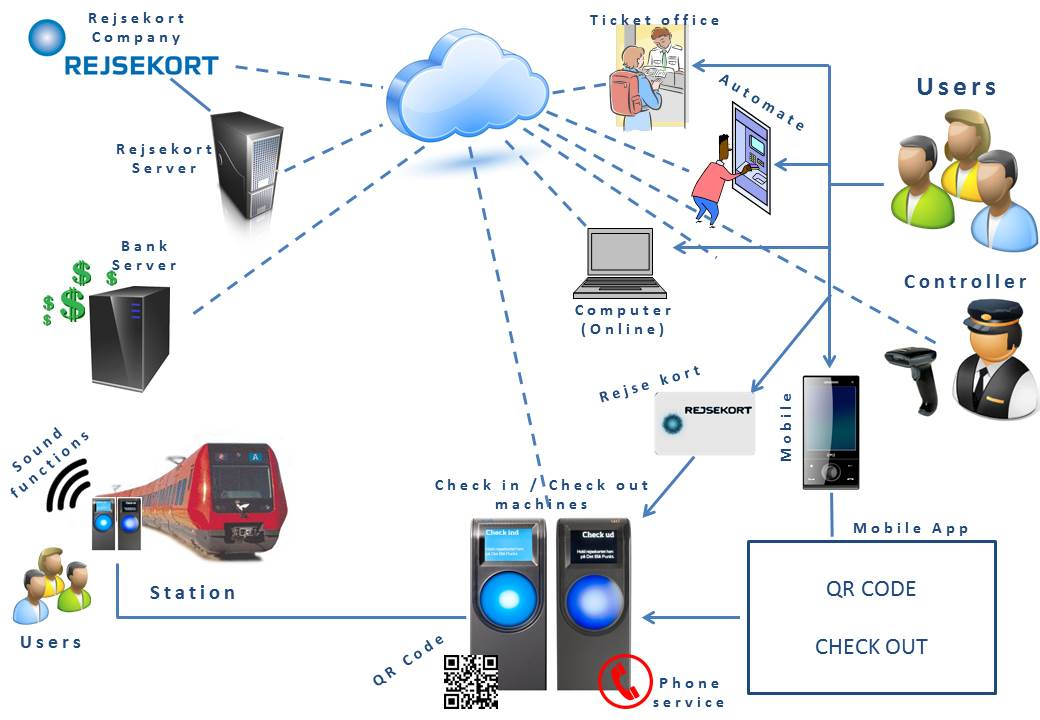
\includegraphics[width=100mm]{graphics/Rejse_Kort_Rich_Picture_2nd.jpg}
\caption{Class Diagram Draft}
\label{overflow}
\end{figure}

\section*{Class Diagram}

\begin{figure}[ht!]
\centering
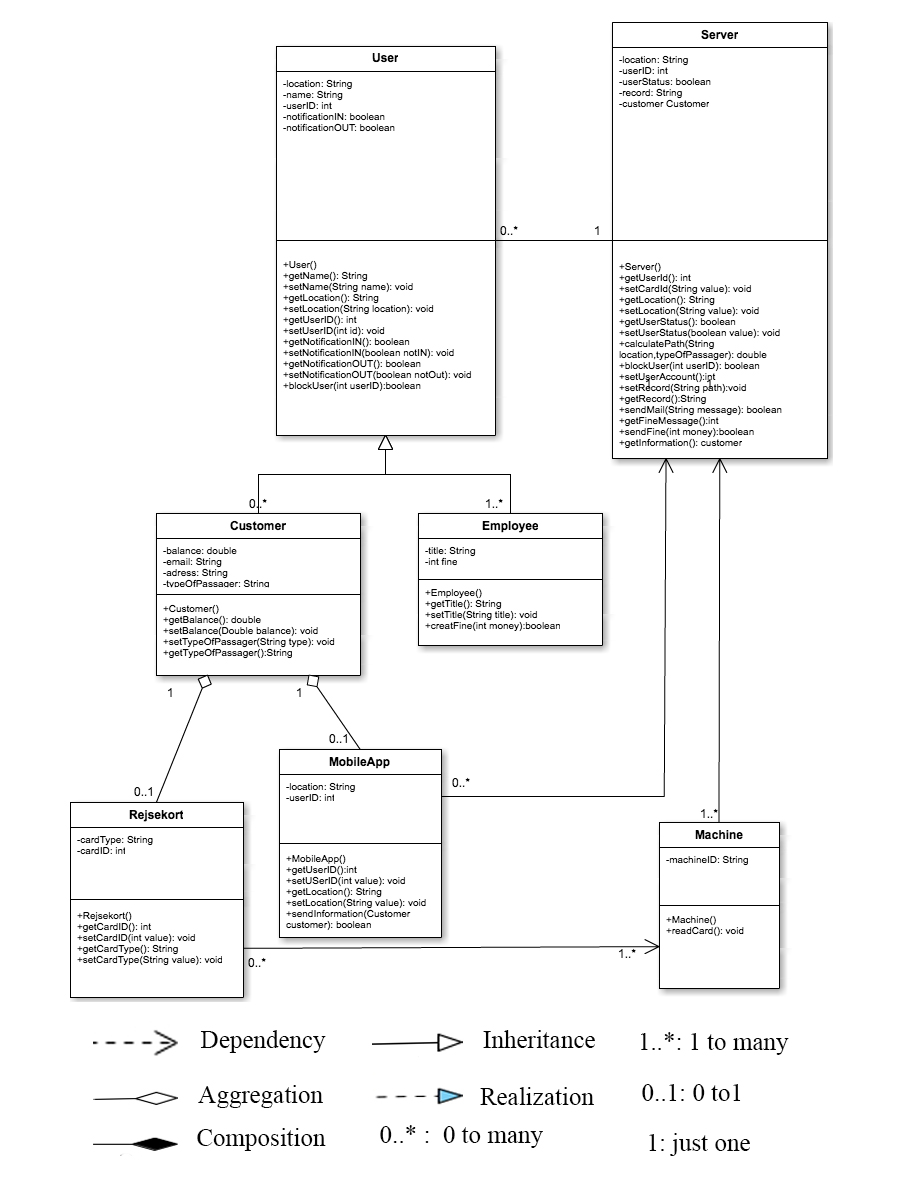
\includegraphics[width=100mm]{graphics/classdiagram.jpg}
\caption{Class Diagram}
\label{overflow}
\end{figure}

\subsection*{Description}

\subsubsection{User}
There are two types of users in this system. They are customers who use the system to travel. And also employee works in the public transport company. And both users can access to users’ status(check in/out) and location (zone area).

\subsubsection{Customer}
Customers have more functions than the User class. Customer has the balance value. That means customers can check and charge their own balance accounts. The customers have two ways to use the system. One is rejsekort. Another is mobile app.

\subsubsection{Employee}
The employees who use the system are ticket controllers. They can only access to users’ ID, status and location.

\subsubsection{MobileApp}
Mobile app can get users’ ID, status, location(with GPS) and return all the data back to the server. Users also get balance data from server.

\subsubsection{Rejsekort}
Customers can always use the card to check in/out and check balance through the machines in the station. The card contains customers’ ID, name and etc.

\subsubsection{Machine}
Machines are located all the stations and buses in Denmark. The machines can read rejsekort. And they can send customers’ informations and location back to server. And the machines can also get customers’ balance base on customers’ ID from the the server.

\subsubsection{Server}
The server contains all the customers’ ID, status, location, balance and customers’ information. The server can receive all the data from the mobile and the machines. The server can also calculate the price base on check in/ out location and charge that price from balance account. 